\chapter{Обзор предметной области}
\label{chapter_review}

\section{Эволюционные алгоритмы}
Эволюционный алгоритм(ЭА)~\cite{skobtsov, eiben-ea} является методом решения задач оптимизации. Данный подход основан на идеях, заимствованных из биологической эволюции: естественный отбор, мутация, скрещивание и наследование признаков. Каждая итерация алгоритма характеризуется набором особей, называемым поколением. Начальное поколение обычно формируется случайным образом. На множестве особей вводят функции приспособленности, чтобы количественно оценивать, насколько данная особь близка к верному решению. Наиболее приспособленные особи имеют большую вероятность быть выбранными для создания нового поколения. При помощи оператора скрещивания (кроссовера) по двум особям текущего поколения создается новая особь для следующего поколения. Оператор мутации вносит в особь малые случайные изменения. Общая схема эволюционного алгоритма представлена на листинге~\ref{ea_scheme}.

\begin{algorithm}[h!]
\caption{Общая схема эволюционного алгоритма}
\label{ea_scheme}
\begin{algorithmic}[1]
  \STATE {Создать начальное поколение}
  \STATE {Вычислить значение функции приспособленности для каждой особи}
  \WHILE {(условие останова эволюционного алгоритма не выполнено)}
    \STATE {Выбирается подмножество особей текущего поколения}
    \STATE {Применяя операторы мутации и кроссовера к выбранным особям, создаются новые особи}
    \STATE {Вычисляется значение функции приспособленности для созданных особей}    
    \STATE {Путем замены новыми особями наименее приспособленных в текущем поколении формируется новое поколение}
  \ENDWHILE  
\end{algorithmic}
\end{algorithm}

В качестве критерия останова часто используют следующие условия~\cite{mitchell-ga}:
\begin{itemize}
 \item найдено верное решение;
 \item достигнуто заданное количество поколений;
 \item превышено заданное время работы;
 \item превышено заданное число вычислений функции приспособленности;
 \item за заданное число поколений не произошло улучшение решения.
\end{itemize}

Эволюционные алгоритмы применяются для решения задач оптимизации, к которым точные алгоритмы не применимы. Стоит отметить, что эффективность работы эволюционного алгоритма сильно зависит от выбора значений его параметров, таких как вероятность мутации, вероятность скрещивания, число особей в поколении. Значения параметров зависят не только от эволюционного алгоритма, но и от решаемой задачи оптимизации. Подбор параметров может осуществляться до запуска эволюционного алгоритма. Однако оптимальные значения параметров могут изменяться в ходе работы алгоритма. Поэтому необходим метод адаптивной настройки параметров в процессе оптимизации.

\section{Обзор существующих методов настройки параметров ЭА}

Рассмотрим формальную постановку задачи адаптивной настройки параметров ЭА. Имеется набор $\{v_1, ..., v_n\}$ из $n$ параметров ЭА, каждый из которых может принимать значения из некоторого дискретного набора или из непрерывного интервала значений. Целью алгоритма является выбор таких значений параметров $v_i$, чтобы ЭА работал наиболее эффективно.

Большинство алгоритмов адаптивной настройки параметров ЭА можно отнести к классу методов сопоставления  вероятности (probability matching techniques), в которых вероятность выбора значения параметра пропорциональна эффективности его применения~\cite{eiben_1}. В данной работе использовался один из наиболее эффективных алгоритмов данного класса, называемый \textit{earpc}.

\subsection{Метод earpc}
\label{earpc}
В методе \textit{earpc}~\cite{earpc} выбор значений параметров происходит независимо друг от друга. В данном методе для выбора значения параметра диапазон допустимых значений делится во время работы алгоритма на два подинтервала.

Схема работы алгоритма \textit{earpc} представлена на листине~\ref{earpc_scheme}. Будем называть назначением параметров набор $\textbf(v)$ подобранных значений параметров $(v_1, .., v_n)$. В ходе работы алгоритма каждому назначению параметров $\textbf(v)$ соответствует некоторый функционал качества $q(\textbf(v))$. Выбор новых значений параметров осуществляется следующим образом. Ранее используемые назначения параметров разбиваются на два кластера $c_1$ и $c_2$, например, с помощью алгоритма \textit{k-means}. Затем для каждого параметра $v_i$ интервал его допустимых значений разбивается на два подинтервала. Для этого необходимо выбрать подходящую точку разбиения. Для этого все ранее используемые назначения параметра $v_i$ сортируются по возрастанию. В качестве кандидатов на точку разбиения рассматриваются средние значения между двумя соседними назначениями в полученной упорядоченной последовательности. Для каждого кандидата $s$ на точку разбиения  множество ранее используемых назначений разбивается в соответствии с $s$ на два множества $p_1$ и $p_2$. Во множестве $p_1$ находятся все ранее используемые назначения параметра $v_i$, меньшие или равные $s$, а в множестве $p_2$ находятся все ранее используемые назначения параметра $v_i$, большие $s$. 
Обозначим $c_i(p_j)$ -- подмножество $p_j$, где $i, j \in \{1, 2\}$,  соответствующее кластеру $c_i$. Для каждого разбиения по формуле~(\ref{entropy}) считается \textit{энтропия}. В качестве итоговой точки разбиения $s$ выбирается та, при которой полученная энтропия минимальна. Для множеств $p_1$ и $p_2$ считается среднее качество $Q_1$ и $Q_2$ соответственно. Множеству $p_1$ соответствует интервал $[v_{min}, s]$, а множеству $p_2$~-- интервал $(s, v_{max}]$, где $v_{min}$ и $v_{max}$ нижняя и верхняя границы диапазона допустимых значений параметра $v_{i}$ соответственно. Из двух данных интервалов значений случайным образом выбирается один, при этом вероятность выбора первого интервала пропорциональна $Q_1$, а второго -- $Q_2$. Затем значение параметра $v_i$ случайным образом выбирается из соответствующего множества. 

\begin{align}
\label{entropy}
e_{p_1} & = -\frac{|c_1(p_1)|}{|p_1|}ln(\frac{|c_1(p_1)|}{|p_1|}) -\frac{|c_2(p_1)|}{|p_1|}ln(\frac{|c_2(p_1)|}{|p_1|}), \nonumber \\
e_{p_2} & = -\frac{|c_1(p_2)|}{|p_2|}ln(\frac{|c_1(p_2)|}{|p_2|}) -\frac{|c_2(p_2)|}{|p_2|}ln(\frac{|c_2(p_2)|}{|p_2|}), \\
H & = \frac{|p_1|}{|c_1|}e_{p_1} + \frac{|p_2|}{|c_2|}e_{p_2} \nonumber 
\end{align}


\begin{algorithm}[h!]
    \caption{Алгоритм \textit{earpc} в случае деления на два подинтервала.}
    \label{earpc_scheme}
    \begin{algorithmic}[1]
        \STATE {Ранее выбранные назначения параметров $\{(v_1, .., v_n)\}$ разбиваются на два кластера $c_1$ и $c_2$ с помощью алгоритма \textit{k-means}.}
	\FOR {параметр $v_i$}
	    \STATE {Отсортировать назначения параметров по значению \textit{i}-ого}
	    \STATE {$H_{best} \gets \infty$}
	    \FOR {точка разбиения $s = \frac{v_{ij} + v_{i(j+1)}}{2}$}
	      \STATE {Разбить назначения в соответствии с точкой разбиения \textit{s} на множества $p_1$ и $p_2$}
	      \STATE {Рассчитать энтропию \textit{H} разбиения по точке \textit{s} по формуле~(\ref{entropy})} 
	      \IF {$H_{best} < H$}
		\STATE {$H_{best} \gets H$}
		\STATE {Запомнить множества $p_1$ и $p_2$}
	      \ENDIF
	    \ENDFOR
	    \STATE {$Q_1 = \frac{1}{|p_1|}\sum\limits_{\textbf{v} \in p_1}{q(\textbf{v})}$, $Q_2 = \frac{1}{|p_2|}\sum\limits_{\textbf{v} \in p_2}{q(\textbf{v})}$}
	    \STATE {Случайным образом выбрать интервал значений, при этом вероятность выбора первого пропорциональна $Q_1$, а второго -- $Q_2$}
	    \STATE {Случайным образом выбрать значение параметра $v_i$ из выбранного интервала}
	\ENDFOR
    \end{algorithmic}
\end{algorithm}

Недавно был предложен эффективный метод настройки параметров ЭА с помощью обучения с подкреплением. Однако сравнение эффективности применения данного метода и алгоритма \textit{earpc} не проводилось. В данной работе проводится сравнение данных подходов, а также предлагается новый метод адаптивного выбора параметров ЭА. Далее рассматриваются основные принципы работы алгоритмов обучения с подкреплением и метод, предложенный \textit{Karafotias et al}.

\subsection{Обучение с подкреплением}
\label{rl}
Алгоритмы обучения с подкреплением~\cite{sutton,gosavi} часто используются для выбора стратегий поведения в интерактивной среде. Большинство таких алгоритмов не требуют заранее подобранных тестовых примеров, так как их обучение происходит одновременно с применением накопленного опыта.

\begin{figure}
    \centering
    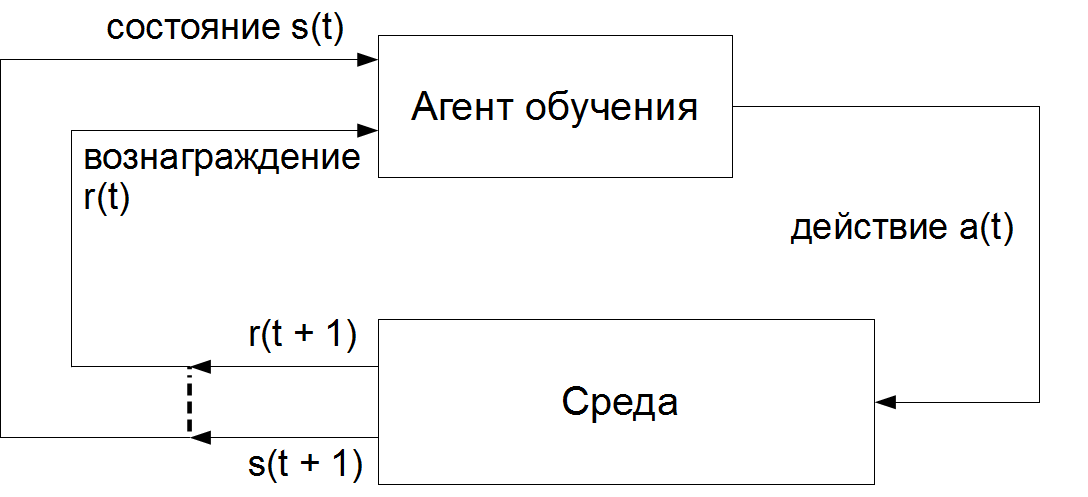
\includegraphics[width=0.6\textwidth]{rl-scheme.png}
    \caption{Схема алгоритма обучения с подкреплением.}
    \label{rl_scheme}
\end{figure}

Принцип работы алгоритма обучения с подкреплением представлен на схеме~\ref{rl_scheme}. У агента есть некоторый набор возможных действий. На каждом шаге алгоритма агент воздействует на среду, которая находится в некотором состоянии, выбирая одно из возможных действий и применяя его к среде. В следствие этого среда может перейти в новое состояние. За выбор действия агент получает численную награду. Задачей агента является максимизация суммарной награды. Действие, выбранное агентом, определяет не только полученную награду, но и состояние, в которое перейдет среда после его применения.

Задачу обучения с подкреплением в большинстве случаев можно описать как \textit{марковский процесс принятия решений}. Для этого необходимо определить:

\begin{itemize}
    \item дискретное множество состояний среды $S$;
    \item дискретное множество действий агента $A$;
    \item функцию награды $R : S \times A \rightarrow \mathbb{R}$;
    \item функцию переходов $T : S \times A \times S \rightarrow \mathbb{R}$ При этом $T(s, a, s')$ определяет вероятность перехода из состояния $s$ в состояние $s'$ после применения действия $a$.
\end{itemize}

Выделяют класс алгоритмов обучения с подкреплением, строящих модель среды, которые используют функцию награды $R$ и функцию переходов \textit{T} для определения стратегии поведения. В частности, возможны стратегии в которых алгоритм будет получать незначительную награду в течение некоторого времени, чтобы достичь некоторого состояния среды, которому соответствует большая ожидаемая награда. В рамках данной работы такие алгоритмы не рассматривались.

\subsubsection{Q-обучение}

Алгоритм $Q$-обучения~\cite{systems, watkins} относится к классу алгоритмов обучения с подкреплением не строящих модель среды. Псевдокод алгоритма представлен на листинге~\ref{q_learning}. Во время работы алгоритма аппроксимируется функция полезности $Q : S \times A \rightarrow \mathbb{R}$, которая описывает ожидаемую награду за действие $a$ в состоянии $s$. Для расчета значений $Q$ обычно используют \textit{TD}-обучение(temporal difference learning). При этом значения $Q$ изменяются по формуле $Q(s, a) = Q(s, a) + \alpha (\gamma Q(s', a') - Q(s, a))$, где $\alpha$~-- скорость обучения, $\gamma$~-- дисконтный фактор.

Выбор действия определяется стратегией исследования среды. Одна из самых простых стратегий - \textit{жадная} заключается в том, чтобы выбирать действие, за которое самое большое ожидаемое вознаграждение, т.е. $\argmax\limits_a{\{Q(s, a)\}}$. Однако в таком случае агент склонен выбирать локально максимальное значение награды, недостаточно исследовав среду. Для улучшения жадной стратегии можно выбирать с вероятностью $\varepsilon$ случайное действие, иначе -- действие с максимальной ожидаемой наградой. Такая стратегия называется $\varepsilon$\textit{-жадной}. При этом значение $\varepsilon$ может меняться во время работы алгоритма, что позволяет перейти от исследования среды к применению накопленного опыта.

\begin{algorithm}[h!]
    \caption{Алгоритм Q-обучения с $\varepsilon$-жадной стратегией исследования среды.}
    \label{q_learning}
    \begin{algorithmic}[1]
    \REQUIRE  
        $\varepsilon$ --- вероятность выбора случайного действия;
        $\alpha$ --- скорость обучения;
        $\gamma$ --- дисконтный фактор.
    \STATE {Инициализировать $Q(s, a)$ для всех $s \in S$, $a \in A$}
    \WHILE{{(не достигнуто условие останова)}}
        \STATE {Получить состояние среды $s$}
        \STATE $p \gets ${ случайное вещественное число} $\in [0, 1]$
        \IF {($p \leq \varepsilon$)}
            \STATE $a \gets \arg \max_{a}{Q(s,a)}$
        \ELSE 
            \STATE $a \gets$ { случайное действие } $\in A$
        \ENDIF
        \STATE {Применить действие $a$ к среде}
        \STATE {Получить от среды награду $r$ и состояние $s'$}
        \STATE $Q(s,a) \gets Q(s,a) + \alpha(r + \gamma \max_{a'}{Q(s',a') - Q(s, a))}$
    \ENDWHILE
    \end{algorithmic}
\end{algorithm}

\subsection{Настройка параметров ЭА как задача для обучения с подкреплением}
Рассмотрим задачу выбора параметров эволюционного алгоритма, как задачу, решаемую при помощи обучения с подкреплением~\cite{eiben_2}. В качестве среды выступает эволюционный алгоритм. Агент совершает действие~-- выбор значений настраиваемых параметров, таких как вероятность мутации или кроссовера. Затем среда генерирует следующее поколение особей, используя выбранные значения параметров ЭА, и переходит в новое состояние. Награда, возвращаемая агенту средой, является некоторой функцией от значений оптимизируемой функции~-- функции приспособленности, вычисленных на особях текущего и предыдущего поколений.

Значения параметров ЭА лежат в заданном интервале значений. Таким образом, чтобы установить значение параметра ЭА, агент должен выбрать некоторое значение из заданного интервала. Обычно эту задачу дискретизируют, разделяя диапазон допустимых значений параметра на подинтервалы. Каждый из подинтервалов соответствует действию агента. Совершив действие~-- выбор подинтервала, агент в качестве значения параметра устанавливает случайное значение из выбранного подинтервала. Разбиение на интервалы можно делать априорно, то есть разбиение диапазона значений происходит до запуска алгоритма и не меняется в процессе его работы. Однако для некоторых методов адаптивной настройки параметров было показано, что изменение разбиения во время работы способствует улучшению работы алгоритма~\cite{arpc, earpc}. В частности, значение параметра можно подобрать тем точнее, чем меньше шаг разбиения. В то же время это усложняет задачу выбора оптимального подинтервала. Существующие методы настройки параметров ЭА с помощью обучения с подкреплением используют априорное разбиение.

\subsection{Метод, предложенный Karafotias et al.}
\label{karafotias}

На конференции \textit{GECCO 2014} \textit{Karafotias et al}. предложили метод~\cite{karafotias} подбора параметров ЭА на основе обучения с подкреплением, в котором множество состояний среды формируется во время работы алгоритма, а множество действий задается до запуска алгоритма.

В качестве алгоритма обучения с подкреплением используется $Q$-обучение с $\varepsilon$-жадной стратегией исследования среды.
Предположим, что число настраиваемых параметров равно $k$. Диапазон допустимых значений настраиваемого параметра $v_i$ делится на $m_i$ интервалов до начала работы алгоритма. Действием является выбор интервалов, из которых будет случайно выбрано значение параметра, для всех настраиваемых параметров и обозначается как $b_1, b_2, \ldots, b_k$, где $b_i, 0 < b_i <= m_i$ -- номер интервала для параметра $v_i$. Таким образом число допустимых действий агента в каждом состоянии равно $\prod\limits_{i = 1}^k{m_i}$. Отметим, что действием агента осуществляется одновременный выбор значений для всех параметров. 

Функции награды для ЭА, максимизирующего функцию приспособленности, задается формулой~(\ref{reward}), где $f_t$ -- лучшее значение функции приспособленности, полученное на \textit{t}-ой итерации.
\begin{equation}
\label{reward}
R = c(\frac{f_{t+1}}{f_t} - 1)
\end{equation}
Для ЭА, которые не ухудшают лучшее известное решение, функция награды неотрицательна. Стоит отметить, что значение функции приспособленности зачастую остается неизменным несколько итераций подряд. В самом деле, чтобы награда была положительная, необходимо улучшить лучшую известное значение функции приспособленности. Чтобы замедлить скорость обучения при нулевой награде менялся коэффициент скорости обучения $\alpha$. А именно:
\begin{align*}
Q(s,a) &= Q(s,a) + \alpha(r)(r + \gamma \max_{a'}{Q(s',a') - Q(s, a))} \\
\alpha(r) &= \begin{cases}\alpha, &\text{при } r > 0 \\ \alpha_0, &\text{иначе} \end{cases}
\end{align*}
Стоит отметить, что $\alpha_0 \ll \alpha$.

Для выделения состояний среды используются следующие наблюдаемые характеристики ЭА:
\begin{itemize}
    \item генетическое разнообразие;
    \item разнообразие значений функции приспособленности (среднеквадратичное отклонение);
    \item стагнация (число итераций без улучшения текущего значения функции приспособленности);
    \item прирост среднего в поколении значения функции приспособленности.
\end{itemize}

Множество состояний среды строится при помощи \textit{UTree}, описанного далее. 

\subsubsection{Алгоритм UTree}
\label{utree}
Эффективность применения алгоритмов обучения с подкреплением экспоненциально уменьшается с увеличением числа возможных состояний среды. Однако в большинстве задач не все из них являются существенными. Одним из подходов, позволяющих уменьшить размерность множества состояний среды является объединение нескольких несущественных состояний. Таким образом, множество состояний может быть разбито на несколько значимых состояний. 

Одним из алгоритмов объединения состояний является алгоритм \textit{UTree}~\cite{utree}. В алгоритме \textit{UTree} строится дерево, листьями которого являются полученные в результате объединения состояния. Также существует вариант алгоритма \textit{UTree}, применимый в случае непрерывного множества состояний. Отличие от алгоритма \textit{UTree} для дискретного случая заключается в том, что он не требует изначального выделения состояний среды. Состояния среды выделяются автоматически в ходе работы алгоритма \textit{UTree}.

Схема работы алгоритма представлена на листинге~\ref{utree_scheme}. Состояния среды выделяются на основании наблюдаемых параметров среды. По своей структуре алгоритм \textit{UTree} представляет собой дерево решений в узлах которого стоят условия на параметры среды. Каждому листу соответствует состояние s среды алгоритма обучения с подкреплением, ожидаемое значение награды в котором обозначается как $V(s)$, где $V(s) = \max \limits_a Q(s,a)$. Изначально в дереве существует лишь один лист, и таким образом у среды есть единственное возможное состояние $s$, для которого $V(s) = 0$. Алгоритм состоит из двух циклично повторяемых этапов: этапа сбора данных и этапа их обработки. На этапе сбора данных при помощи текущего построенного дерева по параметрам среды $I$ определяется состояние среды алгоритма обучения с подкреплением $s$. Затем агент \textit{жадно} выбирает действие $a$ и сохраняет полученный кортеж $(I, a, I', r)$,где $I$~-- исходные параметры среды, $a$~-- выбранное действие, $I'$ -- параметры среды после применения действия $a$, $r$~-- награда, полученная агентом. Затем на основе полученного опыта агент обновляет значение $Q(s, a)$. На этапе обработки для каждого сохраненного кортежа вычисляется значение $q(I, a) =  r + \gamma V (s')$~-- значение ожидаемой награды после применения действия $a$ к среде с параметрами $I$, где $s'$~-- состояние среды обучения с подкреплением, соответствующее параметрам среды $I'$. Для каждого состояния $s$ при помощи критерия разбиения ищется точка разбиения. Если такая точка найдена, то состояние $s$ разбивается на два новых состояния. Множество сохраненных кортежей $(I, a, I', r)$ распределяется по новым состояниям. Затем рассчитываются $Q(s_1, a)$, $Q(s_2, a)$, $V(s_1)$ и $V(s_2)$. Отметим, что в методе, предложенном \textit{Karafotias et. al}, значения $Q(s, a)$ копировались в состояния $Q(s_1, a)$, $Q(s_2, a)$, то есть пересчета значений ожидаемой награды не производилось.

\begin{algorithm}[h!]
    \caption{Алгоритм \textit{UTree}.}
    \label{utree_scheme}
    \textbf{Фаза обучения}
    \begin{algorithmic}[1]
        \STATE {По параметрам среды \textit{I} найти соответствующее состояние \textit{s}, являющиеся листом дерева решений.}
        \STATE {Выбрать действие (интервал значений параметра): $a = \argmax\limits_{a'}{Q(s, a')}$.}
        \STATE {Применить выбранное действие к среде, получив награду \textit{r}.}
        \STATE {Сохранить переход $(I, a, I', r)$ в состоянии \textit{s}.}
        \STATE {Обновить значение \textit{Q(s, a)} и $V(s) = \max\limits_a{Q(s, a)}$.}
    \end{algorithmic}
    \textbf{Фаза разбиения}
    \begin{algorithmic}[1]
        \FOR {состояния \textit{s}} 
            \FOR {переход $(I, a, I', r)$ в состоянии \textit{s}}
                \STATE {$q(I, a) = r + \gamma V(s')$}
            \ENDFOR
            \STATE С помощью \textit{критерия разбиения} определить параметр среды и его значение, по которому лучше разделить состояние.
            \IF {найдена точка разбиения}
                \STATE Создать два новых состояния $s_1$ и $s_2$.
                \STATE Распределить переходы состояния \textit{s} по состояниям $s_1$ и $s_2$ в соответствии с  разбиением.
                \STATE Рассчитать \textit{Q($s_1$, a)} и \textit{Q($s_2$, a)} по сохраненным переходам.
                \STATE Заменить состояние \textit{s} в дереве решений, на вершину с детьми $s_1$ и $s_2$ и условием выбора, соответствующим точке разбиения.
            \ENDIF
        \ENDFOR
    \end{algorithmic}
\end{algorithm}

\subsubsection{Критерий Колмогорова-Смирнова}
\label{ks_criteria}
В статистическом анализе используют различные критерии однородности для проверки гипотезы о принадлежности двух независимых выборок одному закону распределения. Одним из наиболее используемых непараметрических критериев о проверке однородности двух эмпирических законов распределения является критерий однородности Смирнова~\cite{stephens}.

Эмпирическая функция распределения является приближением теоретической функции распределения, построенное с помощью выборки из него. Пусть $\{X_i\}_{i = 1}^n$ выборка объема $n$ из случайной величины $X$. Эмпирической функцией распределения случайной величины $X$ называется случайная величина $F(x) = \frac{1}{n}\sum\limits_{i = 1}^n{H(x - X_i)}$, где $H$~-- функция Хевисайда. По сути заданная таким образом функция распределения в точке $x$ равна частоте элементов выборки, не превосходящих $x$.

\begin{figure}
    \centering
    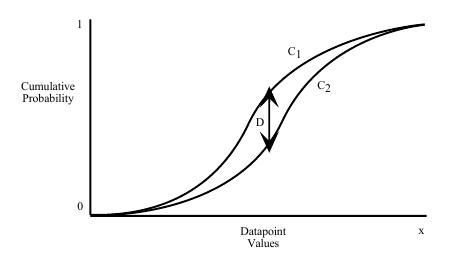
\includegraphics[width=0.6\textwidth]{ks.png}
    \caption{График $F_{a, n}$ и $F_{b, m}$.}
    \label{ks}
\end{figure}

Критерий позволяет найти точку, в которой сумма накопленных частот расхождений наибольшая, и оценить достоверность этого расхождения. В качестве нулевой гипотезы $H_0$ принимается, что две исследуемые выборки подчиняются одному закону распределения случайной величины. Для двух независимых выборок $a$ и $b$, объемами $n$ и $m$ соответственно, строятся эмпирические функции распределения $F_{a, n}$ и $F_{b, m}$. Затем считается значение $\sqrt{\frac{nm}{n + m}}D_{n, m}$, где $D_{n, m} = \sup\limits_x|F_{a, n}(x) - F_{b, m}(x)|$. Если рассчитанное значение превышает квантиль распределения Колмогорова $K_{\alpha}$ для заданного уровня значимости $\alpha$, то нулевая гипотеза $H_0$ отвергается.

\section{Выводы по главе \protect\ref{chapter_review}}

Описаны основные принципы работы алгоритмов обучения с подкреплением, применяющихся в данной работе для настройки параметров ЭА. Приведен обзор существующих методов адаптивной настройки параметров ЭА. Описан способ настройки параметров ЭА как задачи оптимизации, решаемой с помощью алгоритма обучения с подкреплением.
